% This is the University of Chicago Graham School Master of Science in Analytics
% template. Much of it is based on the Reed College LaTeX thesis template.
% Most of the work for the Reec College template was done by Sam Noble (SN),
% Later comments etc. by Ben Salzberg (BTS).
% Additional restructuring and APA support by Jess Youngberg (JY).
% Justin M. Shea (JMS) built on their good open source work.
% Your comments and suggestions are more than welcome:
% please email, them to justinshea@uchicago.edu.
%
% Any line that starts with a percent symbol is a comment.
% They won't show up in the document, and are useful for notes
% to yourself and explaining commands.
% Commenting also removes a line from the document;
% very handy for troubleshooting problems. -BTS
%%
%% Preamble
%%
% \documentclass{<something>} must begin each LaTeX document
% Added by JMS
\documentclass[12pt,oneside]{chicagocapstone}
% END of JMS add
% Packages are extensions to the basic LaTeX functions. Whatever you
% want to typeset, there is probably a package out there for it.
% Check out CTAN to see: http://www.ctan.org/
%%
\usepackage{graphicx,latexsym}
\usepackage{amsmath}
\usepackage{amssymb,amsthm}
\usepackage{longtable,booktabs,setspace}
\usepackage[hyphens]{url}
% Added by CII
\usepackage{hyperref}
\usepackage{lmodern}
\usepackage{float}
\floatplacement{figure}{H}
% End of CII addition
\usepackage{rotating}


% Added by CII (Thanks, Hadley!)
% Use ref for internal links
\renewcommand{\hyperref}[2][???]{\autoref{#1}}
\def\chapterautorefname{Chapter}
\def\sectionautorefname{Section}
\def\subsectionautorefname{Subsection}
% End of CII addition

% Added by CII
\usepackage{caption}
\captionsetup{width=5in}
% End of CII addition

% Added by JMS
\usepackage{mathptmx} % Times New Roman fonts
% End of add by JMS

% Syntax highlighting #22
  \usepackage{color}
  \usepackage{fancyvrb}
  \newcommand{\VerbBar}{|}
  \newcommand{\VERB}{\Verb[commandchars=\\\{\}]}
  \DefineVerbatimEnvironment{Highlighting}{Verbatim}{commandchars=\\\{\}}
  % Add ',fontsize=\small' for more characters per line
  \usepackage{framed}
  \definecolor{shadecolor}{RGB}{248,248,248}
  \newenvironment{Shaded}{\begin{snugshade}}{\end{snugshade}}
  \newcommand{\AlertTok}[1]{\textcolor[rgb]{0.94,0.16,0.16}{#1}}
  \newcommand{\AnnotationTok}[1]{\textcolor[rgb]{0.56,0.35,0.01}{\textbf{\textit{#1}}}}
  \newcommand{\AttributeTok}[1]{\textcolor[rgb]{0.77,0.63,0.00}{#1}}
  \newcommand{\BaseNTok}[1]{\textcolor[rgb]{0.00,0.00,0.81}{#1}}
  \newcommand{\BuiltInTok}[1]{#1}
  \newcommand{\CharTok}[1]{\textcolor[rgb]{0.31,0.60,0.02}{#1}}
  \newcommand{\CommentTok}[1]{\textcolor[rgb]{0.56,0.35,0.01}{\textit{#1}}}
  \newcommand{\CommentVarTok}[1]{\textcolor[rgb]{0.56,0.35,0.01}{\textbf{\textit{#1}}}}
  \newcommand{\ConstantTok}[1]{\textcolor[rgb]{0.00,0.00,0.00}{#1}}
  \newcommand{\ControlFlowTok}[1]{\textcolor[rgb]{0.13,0.29,0.53}{\textbf{#1}}}
  \newcommand{\DataTypeTok}[1]{\textcolor[rgb]{0.13,0.29,0.53}{#1}}
  \newcommand{\DecValTok}[1]{\textcolor[rgb]{0.00,0.00,0.81}{#1}}
  \newcommand{\DocumentationTok}[1]{\textcolor[rgb]{0.56,0.35,0.01}{\textbf{\textit{#1}}}}
  \newcommand{\ErrorTok}[1]{\textcolor[rgb]{0.64,0.00,0.00}{\textbf{#1}}}
  \newcommand{\ExtensionTok}[1]{#1}
  \newcommand{\FloatTok}[1]{\textcolor[rgb]{0.00,0.00,0.81}{#1}}
  \newcommand{\FunctionTok}[1]{\textcolor[rgb]{0.00,0.00,0.00}{#1}}
  \newcommand{\ImportTok}[1]{#1}
  \newcommand{\InformationTok}[1]{\textcolor[rgb]{0.56,0.35,0.01}{\textbf{\textit{#1}}}}
  \newcommand{\KeywordTok}[1]{\textcolor[rgb]{0.13,0.29,0.53}{\textbf{#1}}}
  \newcommand{\NormalTok}[1]{#1}
  \newcommand{\OperatorTok}[1]{\textcolor[rgb]{0.81,0.36,0.00}{\textbf{#1}}}
  \newcommand{\OtherTok}[1]{\textcolor[rgb]{0.56,0.35,0.01}{#1}}
  \newcommand{\PreprocessorTok}[1]{\textcolor[rgb]{0.56,0.35,0.01}{\textit{#1}}}
  \newcommand{\RegionMarkerTok}[1]{#1}
  \newcommand{\SpecialCharTok}[1]{\textcolor[rgb]{0.00,0.00,0.00}{#1}}
  \newcommand{\SpecialStringTok}[1]{\textcolor[rgb]{0.31,0.60,0.02}{#1}}
  \newcommand{\StringTok}[1]{\textcolor[rgb]{0.31,0.60,0.02}{#1}}
  \newcommand{\VariableTok}[1]{\textcolor[rgb]{0.00,0.00,0.00}{#1}}
  \newcommand{\VerbatimStringTok}[1]{\textcolor[rgb]{0.31,0.60,0.02}{#1}}
  \newcommand{\WarningTok}[1]{\textcolor[rgb]{0.56,0.35,0.01}{\textbf{\textit{#1}}}}

% To pass between YAML and LaTeX the dollar signs are added by CII
\title{Music Generator}
\author{Terry Wang, Rima Mittal, Joshua Goldberg}
\date{March, 2020} % The month and year that you submit your FINAL draft)
\division{Graham School}
\advisor{Yuri Balasanov}
\institution{University of Chicago}
\degree{Master of Science in Analytics}
% End of CII addition

\department{Continuing Liberal and Professional Studies}

% Added by CII
%%% Copied from knitr
%% maxwidth is the original width if it's less than linewidth
%% otherwise use linewidth (to make sure the graphics do not exceed the margin)
\makeatletter
\def\maxwidth{ %
  \ifdim\Gin@nat@width>\linewidth
    \linewidth
  \else
    \Gin@nat@width
  \fi
}
\makeatother

\renewcommand{\contentsname}{Table of Contents}
% End of CII addition

\setlength{\parskip}{0pt}

% Added by CII
  %\setlength{\parskip}{\baselineskip}
  \usepackage[parfill]{parskip}

\providecommand{\tightlist}{%
  \setlength{\itemsep}{0pt}\setlength{\parskip}{0pt}}


\Abstract{
We propose the application of Deep Learning models to help individuals generate interesting music ideas. The platform has a GAN-based generator. The data used to train the generator are 130,000 midi files across many different genres of music. The algorithmic process is expected to be able to explore more music combinations than any individual, and thus provide a more holistic and creative approach to music creation.

Our work includes a modified version of the python package pretty\_midi, which serves as a midi pre-processing starter package for Deep Learning. Using Generative Adversarial models, we provide insights on predicting pitches and duration to ultimately generate music notes.

\bigskip 
\bigskip
\bigskip

\textbf{Keywords}: Deep Learning, Music Generation, Generative Adversarial Model, Midi Processing

\bigskip 
\bigskip
\bigskip

\textbf{NOTE:} Do not use ``\#'' or ``\#\#'' symbols to start new sections in the abstract section, as one typically would in other r markdown documents. Doing so will result in generating a table of contents entry \emph{prior} to the Introduction, which is not desirable.
}

% Added by JMS
\Executive{
We propose the application of Deep Learning models to help individuals generate interesting music ideas, with the goal of aiding musicians to use these computer-generated musical ideas to enhance their music writing process. The results show limited success in reaching our goal of meaningful musical output, and we include a few ideas for future improvement on the model.

Our main model is a Generative Adversarial Network with two components: the generative model, which takes a Gaussian noise input of length 128 and outputs a numpy array representing a 20-note midi sample; the discriminator, which takes an input of the numpy array representing a 20-note midi sample and outputs a float between 0 and 1, with 1 representing real and 0 fake. For real samples, we used a midi data repository totaling 130,000 midi files across many different genres of music, but for this project specifically we used mostly Baroque music. For generated samples, we use a deep neural network structure that terminates in separate branches for pitches, whose output is a length 128 softmax vector representing the probabilities of the pitches, and duration, whose output is a vector of 2 positive numbers representing the start and end time of the note, for each of the 20 notes generated. This structure seems to perform the best out of the many structures we tried.

Our work includes a modified version of the python package pretty\_midi. We adapted its main engine to pre-process midi files with varying tempo and key changes and write midi files into numpy array, as well as putting the generated numpy array back into the midi format. In addition, we provided an assortment of utility functions and model selections, which we made into a python package together with the pretty\_midi.

\bigskip
\bigskip
\bigskip

\textbf{NOTE:} Like the abstract, do not use ``\#'' or ``\#\#'' symbols to start new sections in the executive summary section. Doing so will result in generating a table table of contents entry \emph{prior} to the Introduction, which is not desirable.
}
% End of JMS add

\Acknowledgements{

}

\Dedication{

}

\Preface{

}


% End of CII addition
%%
%% End Preamble
%%
%
\begin{document}

% Everything below added by CII
  \maketitle

\frontmatter % this stuff will be roman-numbered
\pagestyle{empty} % this removes page numbers from the frontmatter


%% Reorganized by JMS
  \begin{abstract}
    We propose the application of Deep Learning models to help individuals generate interesting music ideas. The platform has a GAN-based generator. The data used to train the generator are 130,000 midi files across many different genres of music. The algorithmic process is expected to be able to explore more music combinations than any individual, and thus provide a more holistic and creative approach to music creation.
    
    Our work includes a modified version of the python package pretty\_midi, which serves as a midi pre-processing starter package for Deep Learning. Using Generative Adversarial models, we provide insights on predicting pitches and duration to ultimately generate music notes.
    
    \bigskip 
    \bigskip
    \bigskip
    
    \textbf{Keywords}: Deep Learning, Music Generation, Generative Adversarial Model, Midi Processing
    
    \bigskip 
    \bigskip
    \bigskip
    
    \textbf{NOTE:} Do not use ``\#'' or ``\#\#'' symbols to start new sections in the abstract section, as one typically would in other r markdown documents. Doing so will result in generating a table of contents entry \emph{prior} to the Introduction, which is not desirable.
  \end{abstract}
 % Added by JMS
  \begin{executive}
    We propose the application of Deep Learning models to help individuals generate interesting music ideas, with the goal of aiding musicians to use these computer-generated musical ideas to enhance their music writing process. The results show limited success in reaching our goal of meaningful musical output, and we include a few ideas for future improvement on the model.
    
    Our main model is a Generative Adversarial Network with two components: the generative model, which takes a Gaussian noise input of length 128 and outputs a numpy array representing a 20-note midi sample; the discriminator, which takes an input of the numpy array representing a 20-note midi sample and outputs a float between 0 and 1, with 1 representing real and 0 fake. For real samples, we used a midi data repository totaling 130,000 midi files across many different genres of music, but for this project specifically we used mostly Baroque music. For generated samples, we use a deep neural network structure that terminates in separate branches for pitches, whose output is a length 128 softmax vector representing the probabilities of the pitches, and duration, whose output is a vector of 2 positive numbers representing the start and end time of the note, for each of the 20 notes generated. This structure seems to perform the best out of the many structures we tried.
    
    Our work includes a modified version of the python package pretty\_midi. We adapted its main engine to pre-process midi files with varying tempo and key changes and write midi files into numpy array, as well as putting the generated numpy array back into the midi format. In addition, we provided an assortment of utility functions and model selections, which we made into a python package together with the pretty\_midi.
    
    \bigskip
    \bigskip
    \bigskip
    
    \textbf{NOTE:} Like the abstract, do not use ``\#'' or ``\#\#'' symbols to start new sections in the executive summary section. Doing so will result in generating a table table of contents entry \emph{prior} to the Introduction, which is not desirable.
  \end{executive}
 % End of JMS




  \hypersetup{linkcolor=black}
  \setcounter{tocdepth}{2}
  \tableofcontents

  \listoffigures

  \listoftables

%% END of Reorganization by JMS

\mainmatter % here the regular arabic numbering starts
\pagestyle{fancyplain} % turns page numbering back on

\hypertarget{phoenixdowncapstone_gitbook-default}{%
\chapter{phoenixdown::capstone\_gitbook: default}\label{phoenixdowncapstone_gitbook-default}}

Placeholder

\hypertarget{problem-statement}{%
\section*{Problem Statement}\label{problem-statement}}
\addcontentsline{toc}{section}{Problem Statement}

\hypertarget{research-purpose}{%
\section*{Research Purpose}\label{research-purpose}}
\addcontentsline{toc}{section}{Research Purpose}

\hypertarget{variables-and-scope}{%
\section*{Variables and Scope}\label{variables-and-scope}}
\addcontentsline{toc}{section}{Variables and Scope}

\hypertarget{writing-tips}{%
\section*{Writing Tips}\label{writing-tips}}
\addcontentsline{toc}{section}{Writing Tips}

\hypertarget{rmd-basics}{%
\section*{R Markdown Basics}\label{rmd-basics}}
\addcontentsline{toc}{section}{R Markdown Basics}

\hypertarget{lists}{%
\subsection*{Lists}\label{lists}}
\addcontentsline{toc}{subsection}{Lists}

\hypertarget{line-breaks}{%
\subsection*{Line breaks}\label{line-breaks}}
\addcontentsline{toc}{subsection}{Line breaks}

\hypertarget{background}{%
\chapter*{Background}\label{background}}
\addcontentsline{toc}{chapter}{Background}

Placeholder

\hypertarget{code-chunks}{%
\subsection*{Code chunks}\label{code-chunks}}
\addcontentsline{toc}{subsection}{Code chunks}

\hypertarget{linked-tables-and-list-of-tables}{%
\subsection*{Linked tables and List of Tables}\label{linked-tables-and-list-of-tables}}
\addcontentsline{toc}{subsection}{Linked tables and List of Tables}

\hypertarget{more-than-r-other-languages}{%
\subsection*{More than R: Other Languages}\label{more-than-r-other-languages}}
\addcontentsline{toc}{subsection}{More than R: Other Languages}

\hypertarget{pressure-plot}{%
\subsection*{Including plots}\label{pressure-plot}}
\addcontentsline{toc}{subsection}{Including plots}

\hypertarget{ref-labels}{%
\subsection*{R Markdown Tables, Graphics, References, and Labels}\label{ref-labels}}
\addcontentsline{toc}{subsection}{R Markdown Tables, Graphics, References, and Labels}

\hypertarget{inline-code}{%
\subsection*{Inline code}\label{inline-code}}
\addcontentsline{toc}{subsection}{Inline code}

\hypertarget{figures}{%
\subsection*{Figures}\label{figures}}
\addcontentsline{toc}{subsection}{Figures}

\hypertarget{footnotes-and-endnotes}{%
\subsection*{Footnotes and Endnotes}\label{footnotes-and-endnotes}}
\addcontentsline{toc}{subsection}{Footnotes and Endnotes}

\hypertarget{methodology}{%
\chapter*{Methodology}\label{methodology}}
\addcontentsline{toc}{chapter}{Methodology}

The methodology section may include the following subsections:
\begin{itemize}
\tightlist
\item
  Data
\item
  Descriptive analyses
\item
  Modeling Framework
\end{itemize}
\hypertarget{methodology-data}{%
\section*{Data}\label{methodology-data}}
\addcontentsline{toc}{section}{Data}

The training data used to train our model is a collection of midi files that was compiled by a Reddit user \href{https://www.reddit.com/r/WeAreTheMusicMakers/comments/3ajwe4/the_largest_midi_collection_on_the_internet/}{see reddit page} and put up for \href{https://mega.co.nz/\#!Elg1TA7T!MXEZPzq9s9YObiUcMCoNQJmCbawZqzAkHzY4Ym6Gs_Q}{download}. There are about 130,000 midi files from a wide range of genres included in this collection. Our training, however, centers around a small subset of the files that are of 4/4 rhythm, in order to reduce the chance of complication from training with a wider range of rhythmic patterns.

In addition, in our pre-processing script, we took steps to ``normalize'' the samples as much as we can, in terms of making the tempo constant as well as transposing all songs to the key of C major (or A minor if in minor key). The efforts to normalize keys is not always successful. In some midi files, tempo and key changes are included as part of the metadata, which we can then extract and edit. But in others, the metadata is not included.

Before diving deeper into the details of our data, it is necessary to introduce the basic structure of midi files. Midi files (.mid) are digital records of musical ``events'' divided into various tracks, where each track contains a voice, an instrument, or a line of melody. For example, a midi file containing piano music might have two tracks representing the notes played by the two hands of the human piano player. Each time the human player plays a note, the midi file would record the following information: at what time is the piano key pressed; at what time is the key released; how hard is the key pressed; what is the pitch bend. After collecting these information for each and every note in a song in a midi file, we will have most of the information needed to reproduce the song in its entirety down to some basic expressive elements. In the midi metadata, some other relevant information is stored, such as tempo, key, tempo changes, etc. Midi files are not music by themselves because they only contain the information needed to produce music - think of it as the digital equivalent of the sheet music. Midi decoders and synthesizers are needed to translate midi files into music.

If we strip the midi file structure down to its most basic elements, it would look something like this:

\textbf{Insert graph 1-1, unable to get DiagrammeR to work for now}

We can reimagine the midi file to be like a dictionary, where each track is indexed by its name, and in each track we have a nice tabular structure of data consisting of the following columns: pitch number, start time, end time, and pitch velocity (we will ignore pitch bend for now). For example, if we look at the first 3 notes played by the right hand in Beethoven's song Moonlight Sonata, we can tabulate them like the following:
\begin{longtable}[]{@{}llll@{}}
\caption{\label{tab:inher} Midi File Structure Example}\tabularnewline
\toprule
Pitch & Start Time & End Time & Pitch Velocity\tabularnewline
\midrule
\endfirsthead
\toprule
Pitch & Start Time & End Time & Pitch Velocity\tabularnewline
\midrule
\endhead
56 & 0.00 & 0.40 & 33\tabularnewline
61 & 0.40 & 0.81 & 26\tabularnewline
64 & 0.81 & 1.21 & 26\tabularnewline
\bottomrule
\end{longtable}
The above table tells us the following: at time 0.00 seconds pitch 56 is played with velocity 33, and the note stopped at time 0.40 seconds; then at time 0.40 seconds pitch 61 is played with velocity 26, and the note stopped at time 0.81 seconds; and so on. We can see clearly how a piece of music can be represented digitally via the midi file structure.

The other thing to note about midi is the data types of the columns above. The \texttt{Pitch} and \texttt{Pitch\ Velocity} columns take only an integer between 0-127. The \texttt{Start\ Time} and \texttt{End\ Time} columns are positive floats to represent the number of seconds since the start of the song. These things will have an impact on the decisions we made about the model structure.

Since the goal of the model is to generate novel melody ideas, we decided to focus only on pitch, start time, and end time from the midi file information, as well as limiting the output of the generator to 20 notes at a time.

For data fed into the model, we use a processing script to rewrite a pre-selected subset of these midi files into numpy arrays in accordance with the above-mentioned structure: each song will be represented by a series of numpy arrays, each representing a track, and each array will have the tabular structure of 130 columns: a 128-length one hot vector for pitch, start time, and end time. We made the decision to only focus on pitch, start time, and end time in order to focus on learning the melody and not expressiveness, as well as to cut down on complexity. We then use another training script to randomly make 20-note samples from the training data and arrange them into a numpy array. We need 20-note samples in order to make sure that the real and fake samples have the same dimensions\footnote{For our discriminator model this is necessary, but there are other model structures available to overcome this problem.}. Therefore, our training dataset has dimensions of (x, 130, 20) where x represents the number of real samples generated for training, the number 130 represents the three columns (pitch, start time, end time), and 20 represents the 20 notes sampled.

\textbf{maybe insert a chart with sample data structure}

One early choice we made to make the pitch a one-hot vector was done out of the observation about the nature of pitches in the Western musical tradition: the meaning of pitches in the musical sense do not exist in a continuum despite their origins in the frequencies. Therefore, it does not make sense to treat them like so. Instead, one-hot encoding pitches will allow us to treat each pitch as independent objects; in addition, our model will be able to output softmax for pitches, therefore leading to pitch probabilities that can be further investigated. However, there are successful music generation models that treat pitches as one number.

\newpage

\hypertarget{methodology-modeling}{%
\section*{Modeling Framework}\label{methodology-modeling}}
\addcontentsline{toc}{section}{Modeling Framework}

\hypertarget{generator}{%
\subsection*{Generator}\label{generator}}
\addcontentsline{toc}{subsection}{Generator}

Our generator is a deep neural network with the following basic structure:
\begin{figure}

{\centering 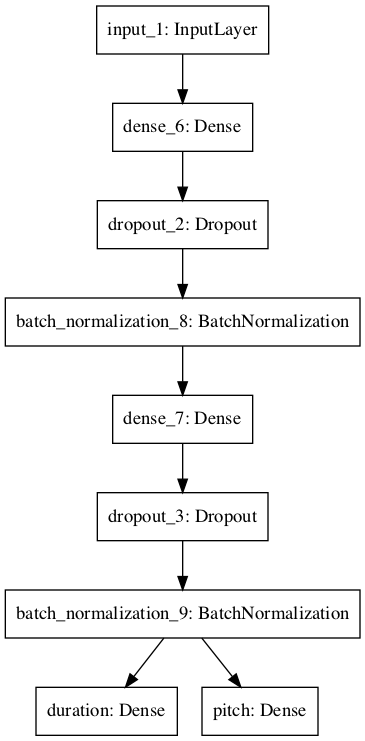
\includegraphics[width=0.3\linewidth]{figure/model_terryjosh} 

}

\caption{museGen Model Structure}\label{fig:unnamed-chunk-1}
\end{figure}
The input of this model is a 128-length vector of standard normal Gaussian noise. The noise will go through 4 layers of dense structure (currently set at 256 nodes) with ReLU activation, dropout, and batch normalization. Then, the model splits in half, one each for pitch and duration generation. The pitch part of the model then upsamples the output from the last layer into 20*128 nodes, where 20 is for the 20 notes to generate, and 128 is for the one-hot vector of pitches. Similarly, we upsample duration from the same layer into 20*2 nodes, where 20 is for the 20 notes to generate and 2 is for start and end times. Afterwards, we have to reshape these nodes into the correct shapes, (20, 128) for pitches and (20, 2) for duration, and apply to the correct axis the corresponding activation functions: softmax for pitch (for pitch onehot), and ReLU for duration (for outputting positive numbers). The generated pitch and duration vectors are then concacted into one single array of dimensions (20, 130) as the output of the model.

Using this modeling structure, we ensure that pitch and duration of one generated music sample is generated by a single model and one single noise input. The dense layers preceding the split in the model will allow the model to learn latent features and rules of music before feeding that latent representation of the final product into the part of the model that turns latent vectors into pitch and duration.

Conventionally, music generation models are

\textbf{Justification of model(s) selected. Identification of dependent and independent variables, per model as well as variable transformations. Feature extraction (if applicable). Discussion of model(s) functional form. Assumptions of model(s) and ways of insuring that assumptions are observed or tested. Assessing model(s) performance and validation.}

Transform \texttt{dose} into a \texttt{factor}. Only three dosage levels are present.
\begin{Shaded}
\begin{Highlighting}[]
\KeywordTok{data}\NormalTok{(ToothGrowth)}
\KeywordTok{colnames}\NormalTok{(ToothGrowth) <-}\StringTok{ }\KeywordTok{c}\NormalTok{(}\StringTok{"length"}\NormalTok{, }\StringTok{"supplement"}\NormalTok{, }\StringTok{"dose"}\NormalTok{)}
\NormalTok{ToothGrowth}\OperatorTok{$}\NormalTok{dose <-}\StringTok{ }\KeywordTok{as.factor}\NormalTok{(ToothGrowth}\OperatorTok{$}\NormalTok{dose)}
\end{Highlighting}
\end{Shaded}
We are most interested in discovering which treatment leads to the optimal tooth growth.
In this vein, we use \texttt{aggregate} function to transform our data and compute the average tooth \texttt{length} by both \texttt{supplement} type and \texttt{dose} size.
\begin{Shaded}
\begin{Highlighting}[]
\NormalTok{groupedTooth <-}\StringTok{ }\KeywordTok{aggregate}\NormalTok{(ToothGrowth, }\DataTypeTok{by=}\NormalTok{ToothGrowth[,}\DecValTok{2}\OperatorTok{:}\DecValTok{3}\NormalTok{], }\DataTypeTok{FUN=}\NormalTok{mean)[,}\DecValTok{1}\OperatorTok{:}\DecValTok{3}\NormalTok{]}

\NormalTok{knitr}\OperatorTok{::}\KeywordTok{kable}\NormalTok{(groupedTooth, }\DataTypeTok{align =} \StringTok{"r"}\NormalTok{, }\DataTypeTok{caption =} \StringTok{"Average tooth length"}\NormalTok{,}
      \DataTypeTok{format =} \StringTok{"latex"}\NormalTok{, }\DataTypeTok{longtable =} \OtherTok{TRUE}\NormalTok{)}
\end{Highlighting}
\end{Shaded}
\begin{longtable}[t]{r|r|r}
\caption{\label{tab:group}Average tooth length}\\
\hline
supplement & dose & length\\
\hline
OJ & 0.5 & 13.23\\
\hline
VC & 0.5 & 7.98\\
\hline
OJ & 1 & 22.70\\
\hline
VC & 1 & 16.77\\
\hline
OJ & 2 & 26.06\\
\hline
VC & 2 & 26.14\\
\hline
\end{longtable}
\newpage

\hypertarget{math-sci}{%
\section*{Math and Science notation}\label{math-sci}}
\addcontentsline{toc}{section}{Math and Science notation}

\TeX~is the best way to typeset mathematics. Donald Knuth designed \TeX~when he got frustrated at how long it was taking the typesetters to finish his book, which contained a lot of mathematics. One nice feature of \emph{R Markdown} is its ability to read \LaTeX~code directly.

Get around math mode's automatic italicizing in LaTeX by using the argument \texttt{\$\textbackslash{}mathrm\{formula\ here\}\$}, with your formula inside the curly brackets. (Notice the use of the backticks here which enclose text that acts as code.)

So, \(\mathrm{Fe_2^{2+}Cr_2O_4}\) is written \texttt{\$\textbackslash{}mathrm\{Fe\_2\^{}\{2+\}Cr\_2O\_4\}\$}.

The \noindent command below does what you'd expect: it forces the current line/paragraph to not indent. See below and examples of commonly used symbols:

\noindent Exponent or Superscript written as \texttt{\$x\^{}2\$} becomes \(x^2\)

\noindent Subscript written as \texttt{\$x\_1\$} becomes \(x_1\)

\noindent Infinity written as \texttt{\$\textbackslash{}infty\$} becomes \(\infty\)

\noindent alpha written as \texttt{\$\textbackslash{}alpha\$} becomes \(\alpha\)

\noindent beta written as \texttt{\$\textbackslash{}beta\$} becomes \(\beta\)

\noindent delta written as \texttt{\$\textbackslash{}delta\$} becomes \(\delta\)

\noindent epsilon written as \texttt{\$\textbackslash{}epsilon\$} becomes \(\epsilon\)

\noindent sigma written \texttt{\$\textbackslash{}sum\_\{i=1\}\^{}n\ f(x)\$} becomes \(\sum_{i=1}^n f(x)\)

\hypertarget{math-examples}{%
\subsection*{Math Examples}\label{math-examples}}
\addcontentsline{toc}{subsection}{Math Examples}

An Ordinary Least Squares model, from \emph{Introductory Econometrics, 6th edition} by Jeffrey M. Wooldridge, page 27.

\[y_i = \beta_0 + \beta_1 x_i + \epsilon_i\]

An infinite distributed lag (IDL) time series model, by Wooldridge, page 633.

\[ y_t = \alpha + \delta_0 z_t + \delta_1 z_{t-1} + \delta_2 z_{t-2} \ldots + \epsilon_t\]

A vector autoregressive (VAR) model, by Wooldridge, page 657.

\[ y_t = \delta_0 + \alpha_1 y_{t-1} + \gamma_1 z_{t-1} + \alpha_2 y_{t-2} + \gamma_2 z_{t-2} \ldots,\]
\newpage

Determinant of a square matrix:

\[\det\left|\,\begin{matrix}%
c_0&c_1\hfill&c_2\hfill&\ldots&c_n\hfill\cr
c_1&c_2\hfill&c_3\hfill&\ldots&c_{n+1}\hfill\cr
c_2&c_3\hfill&c_4\hfill&\ldots&c_{n+2}\hfill\cr
\,\vdots\hfill&\,\vdots\hfill&
  \,\vdots\hfill&&\,\vdots\hfill\cr
c_n&c_{n+1}\hfill&c_{n+2}\hfill&\ldots&c_{2n}\hfill\cr
\end{matrix}\right|>0\]
\bigskip

A regularization problem solved by Jerome Friedman, Trevor Hastie, Rob Tibshirani and Noah Simon, implemented in the \href{https://cran.r-project.org/web/packages/glmnet/index.html}{R package \texttt{glmnet}}.

\[ \min_{\beta_0,\beta} \frac{1}{N}\sum_{i=1}^N w_il(y_i,\beta_0+\beta^Tx_i)+\lambda \left[(1-\alpha) ||\beta||_2^2/2+\alpha||\beta||_1\right]\]

\bigskip

From Lapidus and Pindar, Numerical Solution of Partial Differential Equations in Science and Engineering, page 54.

\[\int_t\left\{\sum_{j=1}^3 T_j \left({d\phi_j\over dt}+k\phi_j\right)-kT_e\right\}w_i(t)\ dt=0, \qquad\quad i=1,2,3.\]

\bigskip

From Lapidus and Pindar, page 145.

\[\int_{-1}^1\!\int_{-1}^1\!\int_{-1}^1 f\big(\xi,\eta,\zeta\big) = \sum_{k=1}^n\sum_{j=1}^n\sum_{i=1}^n w_i w_j w_k f\big( \xi,\eta,\zeta\big).\]

\hypertarget{additional-r-markdown-and-bookdown-resources}{%
\subsection*{Additional R Markdown and bookdown resources}\label{additional-r-markdown-and-bookdown-resources}}
\addcontentsline{toc}{subsection}{Additional R Markdown and bookdown resources}
\begin{itemize}
\item
  \emph{Bookdown} Online Book - \url{https://bookdown.org/yihui/bookdown/}
\item
  \emph{Markdown} Info Sheet - \url{https://github.com/adam-p/markdown-here/wiki/Markdown-Cheatsheet}
\item
  \emph{R Markdown} Reference Guide - \url{https://www.rstudio.com/wp-content/uploads/2015/03/rmarkdown-reference.pdf}
\end{itemize}
\hypertarget{findings}{%
\chapter*{Findings}\label{findings}}
\addcontentsline{toc}{chapter}{Findings}

Placeholder

\hypertarget{findings-descriptive}{%
\section*{Results of descriptive analyses}\label{findings-descriptive}}
\addcontentsline{toc}{section}{Results of descriptive analyses}

\hypertarget{modeling-results}{%
\section*{Modeling results}\label{modeling-results}}
\addcontentsline{toc}{section}{Modeling results}

\hypertarget{results-of-model-performance-and-validation}{%
\section*{Results of model performance and validation}\label{results-of-model-performance-and-validation}}
\addcontentsline{toc}{section}{Results of model performance and validation}

\hypertarget{conclusion}{%
\chapter*{Conclusion}\label{conclusion}}
\addcontentsline{toc}{chapter}{Conclusion}

This section includes a concise summary of the findings. Your summary might be organized by the research objectives or hypotheses. Make sure you address the extent to which research objectives are achieved, and if they are not achieved, explain why. Make sure to interpret your findings in a way that acknowledges the limitations of the research. That is, do not extrapolate the insights derived from your research to situations you have not examined.

\emph{While increasing dosage leads to larger incisor length, the choice of delivery mechanism between Orange Juice and Vitamin C does not seem to make a difference. However, at very low levels, Orange Juice appears more effective, displaying higher average growth.}

\hypertarget{recommendations}{%
\chapter*{Recommendations}\label{recommendations}}
\addcontentsline{toc}{chapter}{Recommendations}

Includes guidelines as to ways in which your results should or could be used in practice. You may discuss other uses of your results, if there are any. The ways to extend your analysis and the benefits of doing so might be included in this section as well.

\appendix

\hypertarget{the-first-appendix}{%
\chapter{The First Appendix}\label{the-first-appendix}}

This first appendix includes all of the R chunks of code that were hidden throughout the document (using the \texttt{include\ =\ FALSE} chunk tag) to help with readibility and/or setup.

\textbf{In section} \ref{pressure-plot}:

\textbf{In section \ref{ref-labels}:}

\hypertarget{a-second-appendix-for-example}{%
\chapter{A Second Appendix, for example}\label{a-second-appendix-for-example}}

\hypertarget{references}{%
\chapter*{References}\label{references}}
\addcontentsline{toc}{chapter}{References}

Placeholder


% Index?

\end{document}
